\chapter{Międzynarodowe zasady turniejowe}
\label{guobiao}
\section{Opis ogólny}
Po wprowadzeniu prawa zakazującego uprawiania hazardu w Chinach w roku 1966
(patrz: strona \pageref{zakaz_1966}), gra w madżonga stała się na powrót legalna
dopiero w 1998 wraz z wprowadzeniem międzynarodowych zasad turniejowych (国标麻将
\pinyin{guóbiāo májiàng} -- patrz: strona \pageref{relegalizacja}).

Autor podjął decyzję o szczegółowym wyjaśnieniu właśnie tych zasad ze względu na
to, że to zgodnie z nimi od 2002 roku rozgrywane są ogólnoświatowe mistrzostwa
gry w madżonga (patrz: strona \pageref{pierwsze_mistrzostwa}).

Treść zasad opisana w dalszej części podrozdziału powstała na podstawie
dokumentu opublikowanego przez Światową Organizację Madżonga (patrz: strona
\pageref{wmo}) 2 kwietnia 2014 roku (Shìjiè Májiàng Zǔzhī 2014), czyli zgodnie
z najnowszą ich wersją. Same zasady mogą być modyfikowane przez organizację w
przyszłości, w związku z czym niektóre informacje zawarte w tym podrozdziale
mogą z czasem stać się nieaktualne.

Niektóre elementy opisanych zasad dotyczą zachowania i ubioru graczy na zawodach
sportowych. Mimo że nie wpływają one bezpośrednio na przebieg rozgrywki, są one
elementem współczesnej kultury gry w madżonga. Poza terenem zawodów mogą one być
stosowane wybiórczo.

\section{Etykieta}
Graczy powinno cechować silne poczucie moralności. Muszą oni grać uczciwie,
przestrzegać osądów arbitrów oraz okazywać szacunek innym graczom. Ponadto,
powinni także ubierać się schludnie i zachowywać uprzejmie wobec innych.

Palenie wyrobów nikotynowych w czasie gry jest zabronione. Zawodnicy nie mogą
nosić lub używać jakichkolwiek produktów, które mogą wpływać na grę.

Arbitrzy muszą przejść specjalne szkolenia oraz wykonywać swoje obowiązki z
powagą, szczerością i uczciwośćią, jak też i zgodnie z obowiązującymi zasadami.

%\pagebreak
\section{Terminologia}
\label{terminologia}
Podstawowe terminy\footnote{Niektóre terminy zostały już pobieżnie
wyjaśnione na potrzeby definicji madżonga (patrz: strony \pageref{zastrzezenia}
i \pageref{definicja}), jednakże tutaj autor wyjaśnia niektóre z nich bardziej
szczegółowo w kontekście zasad turniejowych. Polskie nazwy są tłumaczeniami
przyjętymi przez autora.}:
\begin{itemize}
\item \termin{rozdanie}{盘}{pán}
wszystko, co zachodzi pomiędzy rozdaniem kamieni
a zwycięstwem (lub stwierdzeniem remisu);
\item \termin{wiatr miejsca}{门风}{ménfēng}
każde z miejsc przy stole w danym rozdaniu ma przypisany do siebie jeden z
czterech wiatrów występujących w madżongu (wschodni, południowy, zachodni lub
północny -- patrz też: strona \pageref{wiatry}); miejsca nie są powiązane z
rzeczywistymi kierunkami świata;
\item \termin{przydział miejsc}{定位}{dìngwèi}
przydział miejsc do graczy (czyli tym samym powiązanych z nimi wiatrów) na
początku gry;
\item \termin{diler}{庄家}{zhuāngjiā}
gracz siedzący na miejscu wschodnim;
\item \termin{gracz poboczny}{旁家}{pángjiā}
każdy z graczy nie będących dilerem (czyli gracz południowy, zachodni oraz
północny);
\item \termin{rotacja miejsc}{换位}{huànwèi}
zmiana przypisań wiatrów miejsc do graczy, która może nastąpić po zakończeniu
rozdania;
  \item \termin{obieg}{轮}{lún}
  oznacza sytuację, gdy każdy z graczy już odrzucił
  kamień w turze (wykonał ruch);
\item \termin{runda}{圈}{quān}
w kolejnych rozdaniach każdy z graczy miał
możliwość być dilerem (czyli runda składa się z dokładnie 4 rozdań);
\item \termin{wiatr rundy}{圈风}{quānfēng}
wiatr przypisany do danej rundy (\wiatry);
\item \termin{kompletna gra}{局}{jú}
4 kompletne rundy (w czasie zawodów może
też oznaczać całą rozgrywkę, jaką gracze zdołali przeprowadzić w czasie
przewidzianym na rozegranie 4 rund);
\item \termin{ręka}{手牌}{shǒupái}	%jest już we wstępie wyjaśnione
wszystkie kamienie, jakie w danym momencie posiada gracz (patrz też: strona
\pageref{reka});
\item \termin{sekwens}{顺子}{shùnzi}
dokładnie 3 kolejne kamienie w jednej z talii numerowanych;
\item \termin{trójka}{刻子}{kèzi}
3 identyczne kamienie;
\item \termin{para}{对子}{duìzi}
2 identyczne kamienie;
\item \termin{para ręki}{将牌}{jiàngpái}
2 takie same kamienie znajdujące się na ręce gracza, które są interpretowane 
jako jedyna para przy podliczaniu punktacji; w języku polskim nazywana też
,,głową'' (Polska Liga Mahjonga 2016);
\item \termin{honory}{字牌}{zìpái}
zbiorcze określenie na kamienie wiatrów (\wiatry) i smoków (\smoki); patrz też:
strona \pageref{wiatry};
\item \termin{kamienie terminalne}{幺九牌}{yāojiǔpái}
skrajne kamienie talii numerowanych (czyli kamienie o wartościach 1 oraz 9);
\item \termin{\pinyin{chi}}{吃牌}{chīpái}
wzięcie przez gracza kamienia odrzuconego przez gracza go poprzedzającego
(siedzącego po jego lewej stronie) i użycie go jako dopełnienia własnego
sekwensu;
\item \termin{\pinyin{peng}}{碰牌}{pèngpái}
wzięcie kamienia odrzuconego przez dowolnego innego gracza i użycie go jako
dopełnienia własnej trójki; 
\item \termin{\pinyin{gang}}{杠牌}{gāngpái}
występuje w następujących znaczeniach:
	\begin{itemize}
	  \item cztery identyczne kamienie;
	  \item ekspozycja czterech identycznych kamieni z ręki i dobranie kamienia
	  uzupełniającego;
	  \item dobranie kamienia odrzuconego przez innego gracza i użycie go do
	  własnego \pinyin{ganga} (czterech identycznych kamieni), a następnie dobranie
	  kamienia uzupełniającego;
	\end{itemize}
\item \termin{deklaracja}{报牌}{bàopái}
zgłoszenie \pinyin{chi}, \pinyin{peng}, \pinyin{gang} lub
\hu poprzez wypowiedzenie odpowiedniej nazwy przed wykonaniem akcji;
\item \termin{\hu}{和牌}{húpái}
zwycięstwo w grze (termin ogólny);
\item \termin{kamień uzupełniający kwiat}{补花}{bǔhuā}
po dobraniu jednego z kamieni kwiatów, można go wyeksponować, poprzedzając tę
akcję deklaracją ,,\pinyin{hua}'' (花 \pinyin{huā}), a następnie dobrać kamień;
ów dobrany kamień nazywamy kamieniem uzupełniającym kwiat;
\item \termin{kamień uzupełniający \pinyin{gang}}{补杠}{bǔgāng}
kamień dobierany po deklaracji \pinyin{gang};
\item \termin{czekanie}{听牌}{tīngpái}
stan, w którym graczowi brakuje tylko jednego kamienia do wygranej;
\item \termindwapinyiny{mur}{牌墙}{páiqiáng}{牌城}{páichéng}
kamienie ułożone na środku stołu w kształt kwadratu o wysokości 2 i długości 18
kamieni; czasami zwany też ,,Wielkim Murem'';
\item \termin{\pinyin{zimo}}{自摸和}{zìmōhú}
\hu  poprzez dobranie kamienia z muru;
\item \termin{\pinyin{dian}}{点和}{diǎnhú}
\hu  poprzez dobranie kamienia odrzuconego przez innego gracza;
\item \termin{\pinyin{fan}}{番}{fān}
układ punktowany na ręce gracza, który wygrał rozdanie;
\item \termin{karny kamień}{罚张}{fázhāng}
kamień, który gracz zmuszony jest odrzucić w swojej najbliższej kolejce, jako że
wcześniej omyłkowo go odsłonił;
\item \termin{zwycięski kamień}{单放}{dānfàng}
kamień, na którym zwycięzca rozdania deklaruje \hu; 
\item \terminprostyzpodwojnym{nieprawidłowa liczba kamieni}{zbyt
wiele}{多张}{duōzhāng}{zbyt mało kamieni}{少张}{shǎozhāng}
gracz, który w danym momencie gry nie wykonuje ruchu, powinien mieć rękę
składającą się z dokładnie 13 kamieni (wyjątkiem są kamienie uzupełniające
kwiaty i \pinyin{gangi}); posiadanie nieprawidłowej liczby kamieni
dyskwalifikuje możliwość deklaracji hu w danym rozdaniu;
\item \termin{remis}{荒牌}{huāngpái}
sytuacja, w której kamienie z muru zostały wyczerpane, a żaden z graczy nie
zadeklarował \huend;
\item \termindwapinyiny{fałszywe \hu}{错和}{cuòhú}{诈和}{zhàhú}
sytuacja, w której jeden z graczy zadeklarował \huend, jednakże jego ręka
zgodnie z zasadami nie spełnia wymagań wygranej;
\item \termin{podłoga}{牌池}{páichí}
kwadratowy obszar otoczony murem na środku stołu;
\item \termin{zakryta ręka}{门前清}{ménqiánqīng}
ręka, w której kompozycji właściciel nie używał żadnych kamieni odrzuconych
przez innych graczy;
\end{itemize}

\section{Zestaw do gry}
\label{guobiao_zestaw}
Do gry niezbędne są:
\begin{itemize}
  \item 144 kamienie podzielone na 6 typów i 42 wzory\footnote{Precyzyjny opis
  oznaczeń konkretnych kamieni znajduje się w definicji gry przyjętej na
  potrzeby pracy na stronie \pageref{definicja}.}:
  \begin{itemize}
    \item 3 talie numerowane od 1 do 9, po
    4 egzemplarze każdego wzoru, łącznie 108 kamieni:
    \begin{itemize}
      \item kółka;
      \item bambusy;
      \item liczby chińskie;
    \end{itemize}
    \item kamienie honorów podzielone na 2 talie, łącznie 28 kamieni:
    \begin{itemize}
      \item kamienie wiatrów (\wiatry), po 4 egzemplarze każdego wzoru, łącznie
      16 kamieni;
      \item kamienie smoków (\smoki), po 4 egzemplarze każdego wzoru, łącznie 12
      kamieni;
    \end{itemize}
    \item 8 różnych kamieni kwiatów\footnote{Kamienie pór roku traktowane są
    jako podzbiór kamieni kwiatów.}, po 1 egzemplarzu każdego wzoru:
    \begin{itemize}
      \item wiosna (春 \pinyin{chūn});
      \item jesień (秋 \pinyin{qiū});
      \item lato (夏 \pinyin{xià});
      \item zima (冬 \pinyin{dōng});
      \item śliwa (梅 \pinyin{méi});
      \item orchidea (兰 \pinyin{lán});
      \item bambus (竹 \pinyin{zhú});
      \item chryzantema (菊 \pinyin{jú});
    \end{itemize}
  \end{itemize}
  \item 2 sześcienne kości do gry, których każda ze ścian jest
  oznaczona kropkami w liczbie od 1 do 6, przy czym ściany z 1 i 4 kropkami mają
  oznaczenia czerwone, podczas gdy pozostałe oznaczone są kropkami niebieskimi
  lub czarnymi;
  \item stabilny stół do gry\footnote{Dozwolone jest także używanie
  automatycznych stołów zatwierdzonych przez Światowe Centrum Turniejów
  Madżonga (世界麻将竞赛中心 \pinyin{Shìjiè Májiàng Jìngsài Zhōngxīn}).} w kształcie
  kwadratu o boku długości 80 do 95 centymetrów, którego powierzchnia powinna
  być pokryta warstwą filcu lub innego materiału nie grubszą niż 0,3 centymetra;
  \item krzesła adekwatne do stołu;
  \item notatnik lub urządzenie elektroniczne zatwierdzone przez Światowe
  Centrum Turniejów Madżonga do zapisywania wyników;
  \item oznaczenie wschodniego wiatru miejsca;
  \item oznaczenie ,,\pinyin{pin}'' (品 \pinyin{pǐn}), symbolizujące moralność i
  uczciwość graczy;
  \item oznaczenie ,,cisza'' (静 \pinyin{jìng}), mające przypominać graczom o
  konieczności zachowania ciszy w czasie gry (z wyłączeniem deklaracji i rozmów
  niezbędnych do gry).
\end{itemize}

\section{Cel gry}
Celem gry jest uzbieranie liczby punktów większej od pozostałych graczy
w ciągu wszystkich rozdań składających się na kompletną grę. Punkty
można otrzymywać poprzez ułożenie wygrywającej ręki zanim uda się to któremuś z
pozostałych graczy w danym rozdaniu oraz tracić, gdy dokona tego jeden z
pozostałych zawodników.

\label{wygrywajacareka}
Wygrywająca ręka spełnia następujące wymagania:
\begin{itemize}
  \item składa się z 14 kamieni (opcjonalnie może być powiększona o od 0 do 8
  kamieni kwiatów), czyli 4 grup (trójek, \pinyin{gangów} lub sekwensów) oraz
  pary (za wyjątkiem \pinyin{fan} przyzwalających na inny układ, patrz:
  \pinyin{fan} na stronie \pageref{fan});
  \item jest zgodna z \pinyin{fan} (patrz: \pinyin{fan} na stronie
  \pageref{fan}) o łącznej wartości co najmniej 8 punktów (nie wliczając w to
  punktów za kamienie kwiatów).
\end{itemize}

\section{Przebieg gry}
\subsection{Przygotowanie do gry}
W grze bierze udział dokładnie 4 graczy. Po przygotowaniu sali (umieszczeniu
oznaczeń w odpowiednich miejscach) oraz zestawu do gry, gracze zajmują
przypisane im miejsca przy stole. W czasie zawodów sportowych przypisywane są
one po uprzednim losowaniu przez władze organizujące turniej. W przypadku gier o
mniej oficjalnym charakterze, gracze sami losują miejsca lub zajmują je w
dowolny sposób. %można wrzucić gdzieś metodę losowania wiatrów

Układ wiatrów miejsc przy stole jest ustalony. Diler zasiada na miejscu
wschodnim, następnie w kierunku przeciwnym do ruchu wskazówek zegara po kolei
znajdują się wiatr południowy, zachodni i północny.

\subsection{Budowa muru i podział kamieni}
Gracze obracają wszystkie kamienie stroną z oznaczeniami do dołu po czym
dokładnie je mieszają. Następnie, każdy z zawodników bierze 36 kamieni i buduje
ścianę o długości 18 i wysokości 2 kamieni. W kolejnym kroku gracze ustawiają
swoje ściany w kwadratową formację pośrodku stołu, zwaną dalej ,,murem''.

Aby rozdzielić kamienie z muru pomiędzy graczy, tworząc dla każdego z nich jego
początkową rękę, należy dokonać 2 rzutów kośćmi. Rzutów należy dokonywać na
podłodze pomiędzy 4 ścianami muru z wysokości pomiędzy 10 a 20 centymetrów nad
jej powierzchnią. 

Pierwszy rzut wykonuje diler, sumuje wynik, po czym odlicza poczynając od siebie
w kierunku przeciwnym do ruchu wskazówek zegara. Wybrany w ten sposób gracz
rzuca kośćmi po raz drugi, sumuje wynik wraz z wynikiem poprzedniego
rzutu i odlicza otrzymaną liczbę kamieni poczynając od prawej strony
znajdującego się przed nim boku muru w kierunku zgodnym z kierunkiem ruchu
wskazówek zegara. Za ostatnim odliczonym w ten sposób kamieniem następuje
przełamanie muru i od kolejnego zaczynamy dobieranie kamieni przez graczy.

Zaczynając od dilera, zawodnicy po kolei w kierunku przeciwnym do ruchu
wskazówek zegara trzykrotnie biorą po 4 kamienie, w rezultacie czego każdy z
nich ma ich po 12. Następnie, w tej samej kolejności każdy z graczy dobiera po
jednym kamieniu, z wyjątkiem dilera, który po nich dobiera jeszcze jeden, który
byłby kolejny z kolei (czyli łącznie 2).

Na koniec powyżej opisanego procesu diler powinien mieć 14 kamieni, podczas gdy
pozostali gracze powinni ich mieć po 13. Po przełamaniu muru jego „początkiem”
określa się to jego zakończenie, z którego gracze po kolei dobierali kamienie na
początku gry, natomiast „końcem” nazywa się zakończenie przeciwległe.

Przykład znajduje się na Rysunku \ref{fig:mur}.

\begin{figure}[H]
\centering
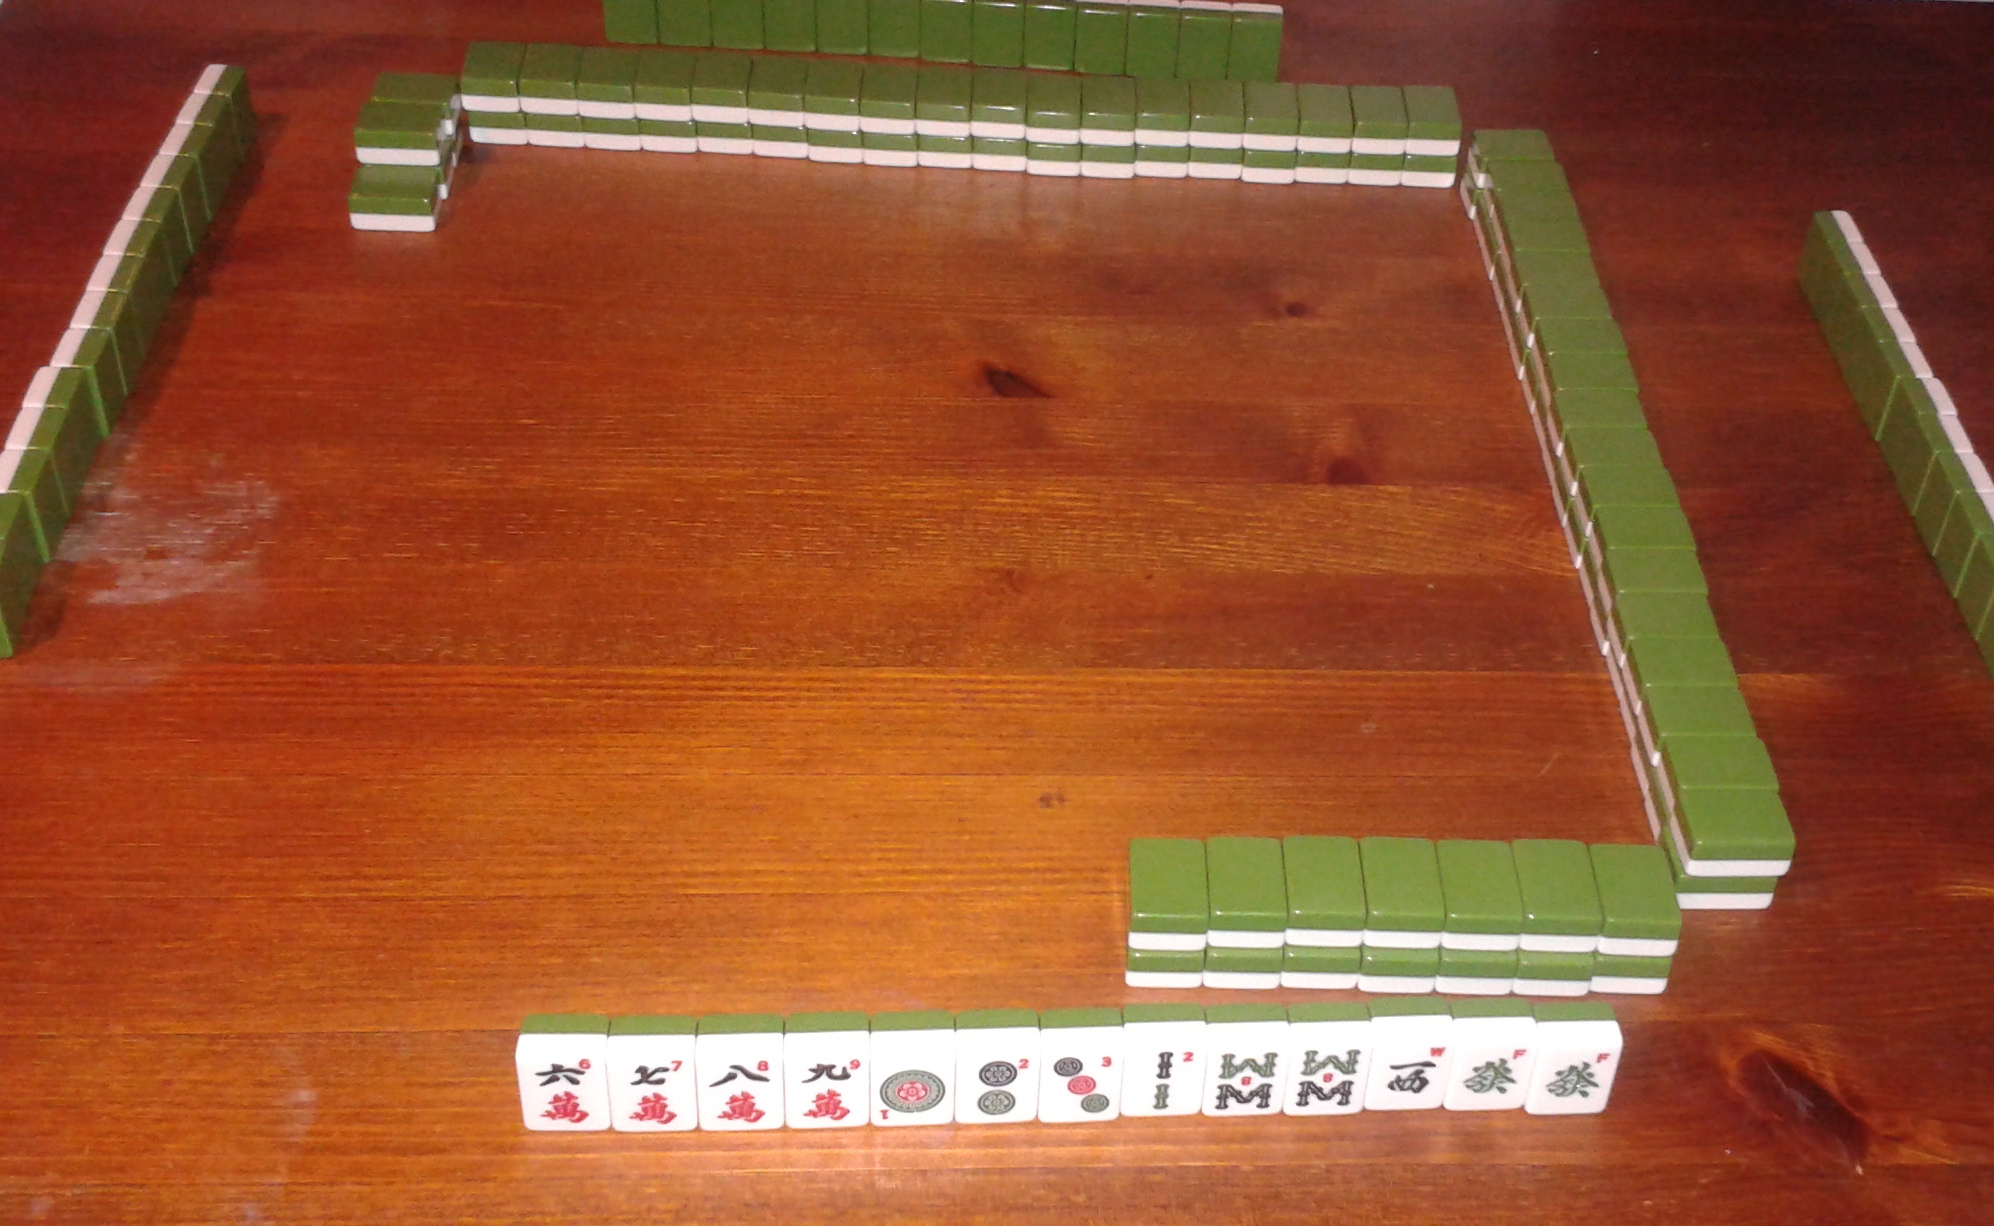
\includegraphics[width=0.75\textwidth]{mur.jpg}
\caption{Przykład sytuacji po zbudowaniu muru i rozdzieleniu kamieni pomiędzy
graczy; źródło: fotografia własna}
\label{fig:mur}
\end{figure}

\subsection{Aranżacja kamieni i deklaracje kwiatów}
Zawodnicy mogą w dowolny sposób przearanżować kamienie w swojej ręce, nie
pokazując ich pozostałym uczestnikom gry. Gracze, którzy w pierwszym przydziale
otrzymali dowolną ilość kamieni kwiatów, mogą zadeklarować \pinyin{hua} (patrz:
deklaracje na stronie \pageref{deklaracje}). Deklaracje
wykonuje się zaczynając od dilera w kierunku przeciwnym do wskazówek zegara.  
 
\subsection{Przebieg tury}
Po rozdzieleniu kamieni i deklaracji kwiatów,  gracze po kolei wykonują ruchy w
swoich turach. Pierwsza tura przysługuje dilerowi, następnie wykonują je gracze
w ruchu przeciwnym do wskazówek zegara aż do zakończenia rozdania (czyli po
kolei w cyklu gracze z przypisanym wiatrem miejsca wschodnim, południowym,
zachodnim, północnym, a następnie ponownie wschodnim).

Każdy z graczy na początku swojej tury dobiera kamień z początku muru (nie
licząc pierwszej tury dilera, który zaczyna z 1 kamieniem więcej), może dokonać
deklaracji kwiatu (jeśli takowy dobrał) lub zakrytego \pinyin{ganga} (patrz:
deklaracje na stronie \pageref{deklaracje}), a następnie deklaruje \pinyin{hu}
lub odrzuca kamień ze swojej ręki (może to być kamień właśnie przez niego dobrany). Tura
nie powinna trwać więcej niż 10 sekund.

Kamienie odrzucone należy ustawiać w rzędach o długości 6 kamieni, od lewej do
prawej, na podłodze pomiędzy ścianami muru. 

Kolejny gracz nie może rozpocząć swojej tury (dobrać kamienia z początku muru)
dopóki jego poprzednik nie odrzucił kamienia. 

Deklaracje wzięcia kamienia odrzuconego (patrz: deklaracje na stronie
\pageref{deklaracje}) powinny nastepować w odstępie kilku sekund od jego
odrzucenia, jeszcze zanim kolejny gracz zdąży rozpocząć swoją turę.

Kolejność tur zostaje zmieniona, a aktualny obieg przerwany i rozpoczęty nowy,
gdy odrzucony kamień zostanie przejęty przez innego gracza przez odpowiednią deklarację.
Wówczas rozpoczyna się tura deklarującego (przy czym zabrany przez niego kamień
zastępuje dobranie kamienia z muru), po nim tura gracza po jego prawej stronie i
tak dalej.

\subsection{Odkryte kamienie}
Po wykonaniu deklaracji \pinyin{peng}, \pinyin{gang} (wariantu odkrytego) lub
\pinyin{chi}, ręka gracza przestaje być zakryta, a przed nią
umieszczone zostają  odpowiednio trójka, \pinyin{gang} lub sekwens. W każdym z
tych 3 przypadków są to kamienie odkryte, a jeden z nich został wcześniej
odrzucony przez jednego z pozostałych graczy. W takim wypadku należy zaznaczyć,
który kamień został zabrany i który z graczy go odrzucił. Dokonuje się tego
poprzez obrócenie owego kamienia o 90 stopni i umieszczenie go:
\begin{itemize}
  \item po stronie prawej, jeśli został on zabrany od gracza po prawej stronie
  deklarującego (Rysunek \ref{fig:meldright});
  \begin{figure}[H]
  \centering
  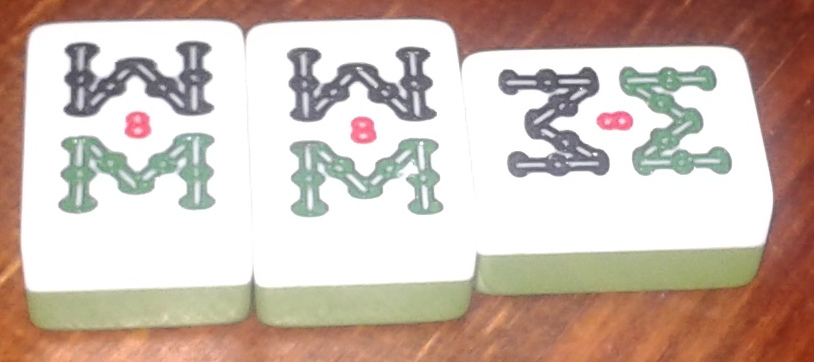
\includegraphics[width=0.50\textwidth]{meld_right.jpg}
  \caption{Przykład zgłoszenia \pinyin{peng} dla trójki złożonej z kamieni o
  numerze 8 z talii bambusów, przypadek dla kamienia zabranego od gracza po
  prawej stronie; źródło:
  fotografia własna}
  \label{fig:meldright}
  \end{figure}
  \item po stronie lewej, jeśli został on zabrany od gracza po lewej stronie
  deklarującego (Rysunek \ref{fig:meldleft});
  \begin{figure}[H]
  \centering
  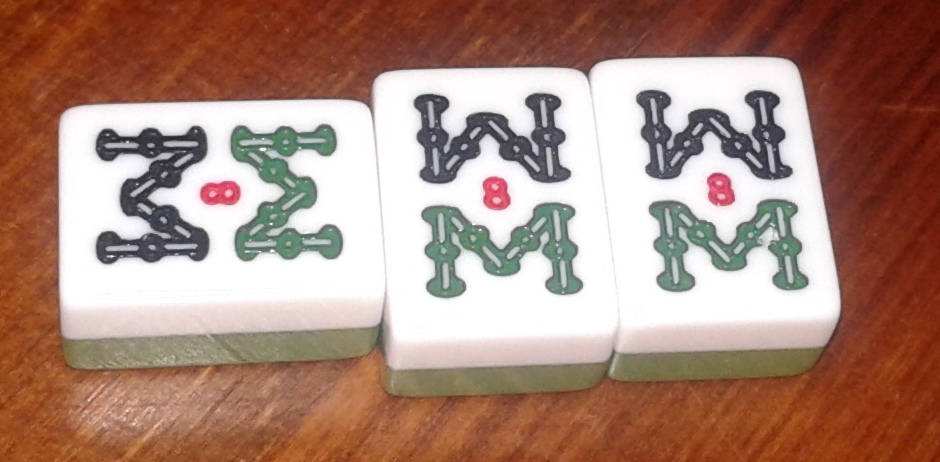
\includegraphics[width=0.45\textwidth]{meld_left.jpg}
  \caption{Przykład zgłoszenia \pinyin{peng} dla trójki złożonej z kamieni o
  numerze 8 z talii bambusów, przypadek dla kamienia zabranego od gracza po
  lewej stronie; źródło: fotografia własna}
  \label{fig:meldleft}
  \end{figure}
  \item pośrodku, jeśli został on zabrany od gracza naprzeciwko deklarującego
  (Rysunek \ref{fig:meldmid}).
  \begin{figure}[H]
  \centering
  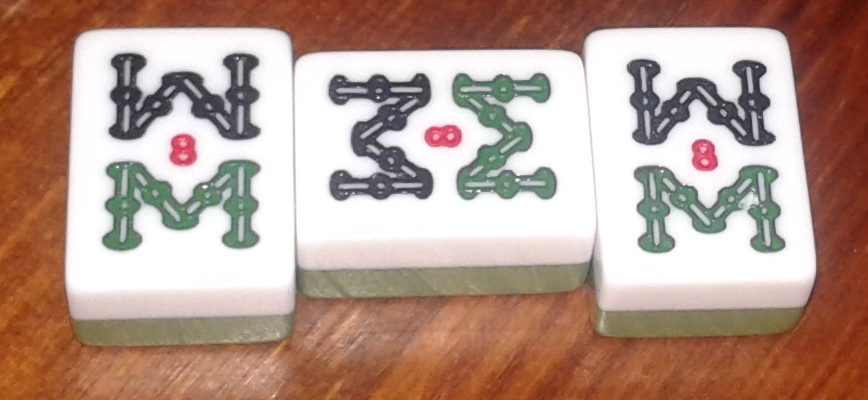
\includegraphics[width=0.45\textwidth]{meld_mid.jpg}
  \caption{Przykład zgłoszenia \pinyin{peng} dla trójki złożonej z kamieni o
  numerze 8 z talii bambusów, przypadek dla kamienia zabranego od gracza
  naprzeciwko; źródło: fotografia własna}
  \label{fig:meldmid}
  \end{figure}
\end{itemize}
% Przykłady znajdują się na Rysunku \ref{fig:meldunki} na stronie
% \pageref{fig:meldunki}.

% \begin{figure}[here]
% \centering
% 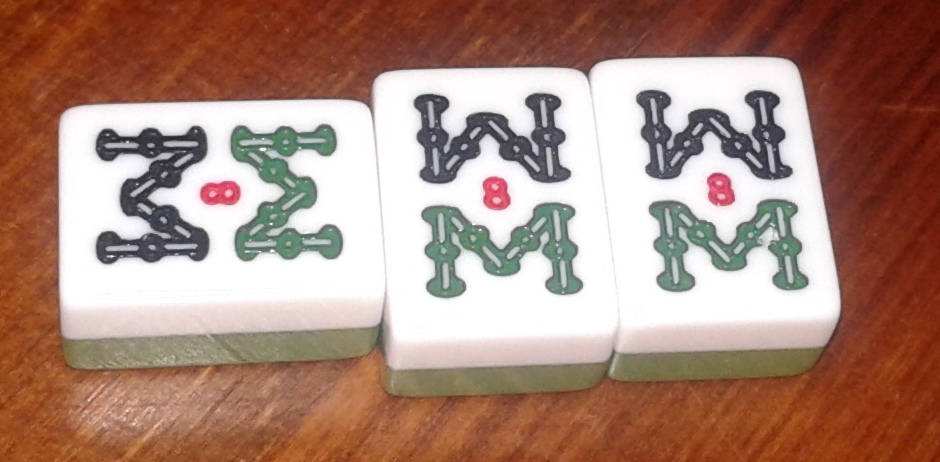
\includegraphics[width=0.75\textwidth]{meld_left.jpg}
% 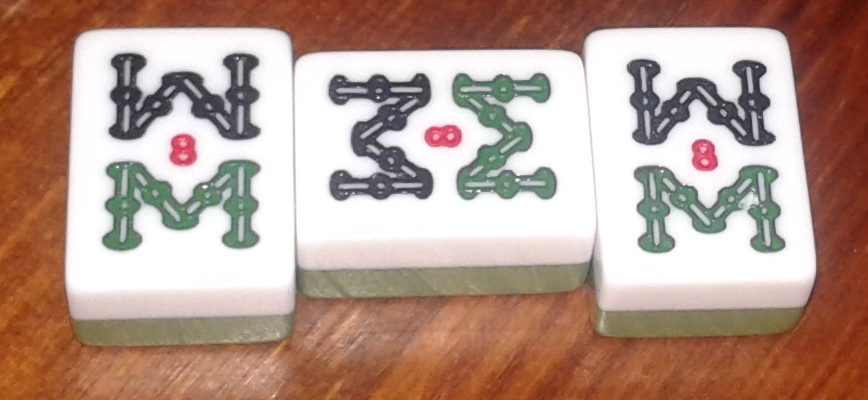
\includegraphics[width=0.75\textwidth]{meld_mid.jpg}
% 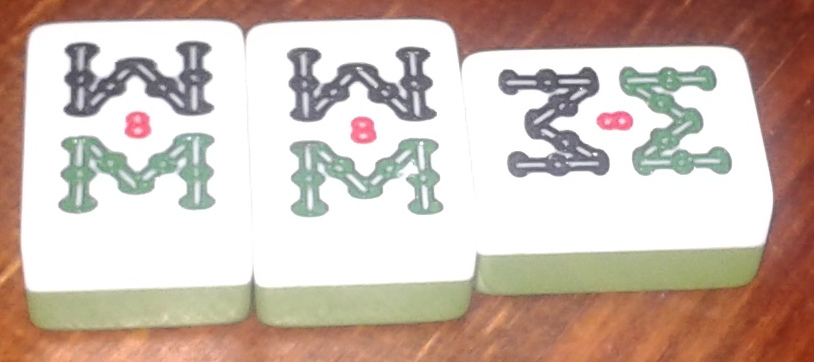
\includegraphics[width=0.75\textwidth]{meld_right.jpg}
% \caption{Przykłady zgłoszeń \pinyin{peng} dla trójki złożonej z kamieni o
% numerze 8 z talii bambusów (odpowiednio dla kamienia dobranego od gracza po
% lewej, naprzeciwko i po prawej stronie gracza); źródło: fotografie własne}
% \label{fig:meldunki}
% \end{figure}

\subsection{Zakończenie rozdania}
Rozdanie kończy się, gdy jeden z graczy zadeklaruje \pinyin{hu} lub zużyte
zostaną wszystkie kamienie w murze (dojdzie do remisu). W przypadku wygranej
zmieniają się punktacje graczy zgodnie z zasadami opisanymi na stronie
\pageref{punktacja}, natomiast przy remisie żaden z graczy nie zyskuje ani nie
traci żadnych punktów. 

Po każdym rozdaniu następuje zmiana dilera, przy czym co 4 rozdania, gdy każdy z
graczy zdążył być dilerem dokładnie raz (na początku każdej nowej rundy),
zachodzi rotacja miejsc (gracze przesiadają się na startowe miejsca przypisane
dla każdej rundy).

Jeśli zakończone rozdanie nie jest ostatnim (czwartym) rozdaniem w rundzie,
nowym dilerem w kolejnym rozdaniu staje się gracz południowy (siedzący po
prawej stronie poprzedniego dilera). Analogicznie, gracz zachodni staje się
południowym, północny -- zachodnim, a wschodni -- północnym.

Jeśli zakończone rozdanie jest ostatnim rozdaniem w rundzie, kończy się
poprzednia runda i zaczyna kolejna (nie licząc sytuacji po zakończeniu rundy
północnej, która jest ostatnią). Na początku nowej rundy następuje zmiana wiatru
rundy. Pierwsza runda to runda wschodnia, a po niej następują kolejno
południowa, zachodnia i północna. Po zakończeniu rundy północnej gra się kończy.

Przy rozpoczęciu nowej rundy następuje rotacja miejsc -- gracze wstają i
przesiadają się zgodnie z układem początkowym przypisanym dla nowej rundy.
Układy te zostały zaprojektowane w taki sposób, aby w przeciągu rozgrywki każdy
z graczy miał tyle samo okazji do deklaracji \pinyin{chi} od każdego z
pozostałych (jako że \pinyin{chi} można deklarować tylko i wyłącznie od gracza
siedzącego po lewej stronie deklarującego). Początkowe układy dla każdej z rund
to:
\begin{itemize}
  \item w rundzie wschodniej (pierwszej) gracze zaczynają na swoich początkowych
  miejscach, czyli gracz A na miejscu wschodnim, gracz B na miejscu
  południowym, gracz C na miejscu zachodnim i gracz D na miejscu północnym;
  \item w rundzie południowej (drugiej) gracz A siada na miejscu południowym,
  gracz B na miejscu wschodnim, gracz C na miejscu północnym i gracz D na
  miejscu zachodnim; 
  \item w rundzie zachodniej (trzeciej) gracz A na miejscu zachodnim, gracz B na
  miejscu północnym, gracz C na miejscu południowym i gracz D na miejscu
  wschodnim; 
  \item w rundzie północnej (czwartej) gracz A na miejscu północnym, gracz B na
  miejscu zachodnim, gracz C na miejscu wschodnim i gracz D na miejscu
  południowym.
\end{itemize}

% gówno prawda, tak jest w riichi, a nie tu
% Jeśli w rozdaniu zwyciężył diler, nie dochodzi do rotacji miejsc i rozgrywane
% jest rozdanie dodatkowe.
% 
% Jeśli w rozdaniu zwyciężył jeden z graczy pobocznych (południe, zachód lub
% północ), następuje rotacja miejsc.
% znowu: riichi 
% Gracz wschodni staje się graczem południowym,
% południowy -- zachodnim, zachodni -- północnym, a północny -- wschodnim.

% Jeśli w wyniku rotacji miejsc nowy gracz wschodni byłby nim po raz drugi w tej
% rundzie (nie licząc rozdań dodatkowych), rozpoczyna się nowa runda (lub, w
% przypadku rundy północnej, zakończona zostaje kompletna gra) i zmienia się
% wiatr rundy. Zmiana wiatru rundy następuje analogicznie do rotacji miejsc, czyli
% po rundzie wschodniej następuje południowa, po południowej -- zachodnia, a po
% zachodniej -- północna. Runda północna jest ostatnią.

\section{Deklaracje}
\label{deklaracje}
W czasie gry przy wszystkich akcjach pozwalających dobrać kamień odrzucony przez
innego gracza (\peng, \dekchi, \hu lub \gang) lub kamień uzupełniający z końca
muru (\pinyin{gang} lub \hua) jest absolutnie obowiązkowym, aby głośno
wypowiedzieć ich deklaracje. Przykładowo, gdy gracz chce dobrać kamień odrzucony przez innego
gracza do własnej trójki, musi głośno powiedzieć ,,\peng'', natomiast gdy chce
go użyć do sekwensu, nie może tego uczynić nie mówiąc ,,\dekchi''. 

Jednakże, gracze nie powinni deklarować nazw kamieni przez nich odrzucanych, a
dyskusja na temat przebiegu gry w jej trakcie jest całkowicie zakazana.

Deklaracje występujące w grze: 
\begin{itemize}
  \item \deklaracja{peng}
  gdy gracz posiada parę danego kamienia (2 jego wystąpienia), a jeden z
  pozostałych uczestników gry odrzuci jego trzeci egzemplarz, posiadacz pary
  może zadeklarować głośno ,,\pinyin{peng}'', zabrać odrzucony kamień, odkryć
  swoją parę i traktować te 3 kamienie jako własną trójkę; deklaracja
  \pinyin{peng} przerywa obieg, zmienia kolejność tur i czyni deklarującego
  aktywnym graczem (musi on w następnej kolejności odrzucić kamień; nie dobiera
  on z muru, jako że otrzymał już kamień wykonując \pinyin{peng});
  \item \deklaracja{gang}
  istnieją 2 sposoby deklaracji \pinyin{gang}:
    \begin{itemize}
    \item odkryty \deklaracja{gang}
    gdy gracz posiada trójkę danego kamienia (3 jego wystąpienia), a jeden z
    pozostałych uczestników gry odrzuci jego czwarty (i tym samym, ostatni)
    egzemplarz, posiadacz trójki może zadeklarować głośno ,,\pinyin{gang}'',
    zabrać odrzucony kamień, odkryć swoją trójkę i traktować te 4 kamienie jako
    własnego \pinyin{ganga} (czwórkę); ten sposób deklaracji \pinyin{gang}
    przerywa obieg, zmienia kolejność tur i czyni deklarującego aktywnym graczem;
    \item zakryty \deklaracja{gang}
    gdy gracz posiada zakryte 4 wystąpienia danego kamienia, może zadeklarować
    głośno ,,\pinyin{gang}'', położyć je zakryte poziomo przed swoją ręką i
    traktować jako \pinyin{ganga} (czwórkę); ten sposób deklaracji zapobiega
    odkryciu ręki;
    \item niezależnie od sposobu deklaracji \pinyin{gang}, po jej wykonaniu
    gracz powinien dobrać kamień uzupełniający z końca muru (w przypadku
    deklaracji odkrytego \pinyin{ganga}, powinien to zrobić przed odrzuceniem
    kamienia);
    \end{itemize}
  \item \deklaracja{chi}
  gdy gracz posiada 2 z 3 kamieni tworzących sekwens, a jeden z pozostałych
  uczestników gry odrzuci 3ci, dopełniający go, można zadeklarować
  głośno ,,\pinyin{chi}'', zabrać odrzucony kamień, odkryć cały sekwens i
  traktować go jako własny; deklaracja
  \pinyin{chi} przerywa obieg, zmienia kolejność tur i czyni deklarującego
  aktywnym graczem (musi on w następnej kolejności odrzucić kamień; nie dobiera
  on z muru, jako że otrzymał już kamień wykonując \pinyin{chi});
  \item \deklaracja{hu}
  gdy gracz ułoży rękę spełniającą kryteria wygranej (patrz: strona
  \pageref{wygrywajacareka}), może głośno zadeklarować ,,\pinyin{hu}'', kończąc
  tym samym rozdanie, odkryć swoje kamienie, a następnie podliczyć należne mu punkty
  (patrz: strona \pageref{punktacja}); można to zrobić, gdy wygrana ręka
  zostanie skompletowana poprzez dobranie wygrywającego kamienia z muru
  (\pinyin{zimo}) lub gdy zostanie on odrzucony przez jednego z pozostałych
  graczy (zabierając go, analogicznie jak przy deklaracji \pinyin{peng} lub
  \pinyin{gang}); w przypadku, gdy 2 lub 3 graczy zadeklaruje \pinyin{hu} na
  jednym kamieniu (odrzuconym przez innego gracza), zwycięża tylko jeden z nich,
  zajmujący miejsce najbliższe w kolejce tur względem gracza odrzucającego
  kamień, na którym padły deklaracje;
  \item \deklaracja{hua}
  gdy gracz dobierze z muru kamień kwiatu (lub zacznie z takowym na ręce
  początkowej w rozdaniu), może zadeklarować głośno ,,\pinyin{hua}'', odkryć
  go, umieścić przed swoją zakrytą ręką, a następnie dobrać kamień uzupełniający
  z końca muru; każdy kamień kwiat zadeklarowany w ten sposób zwiększa końcową
  wartość ręki o 1 punkt.
\end{itemize}

\section{\pinyin{Fan}}
\label{fan}
Istnieje 81 układów punktowanych \pinyin{fan}, z których każdy z nich ma
przypisaną jedną z 12 wartości punktowych: 88, 64, 48, 32, 24, 16, 12, 8, 6, 4,
2 lub 1. Dana ręka
wygrywająca może spełniać więcej niż jedno \pinyin{fan} i aby gracz mógł w
poprawny sposób zadeklarować z nią \pinyin{hu}, muszą one być łącznie warte co
najmniej 8 punktów (z wyłączeniem punktów za kamienie kwiatów).

Istnieje 5 zasad dotyczących interpretacji \pinyin{fan}:
\begin{itemize}
  \item brak powtórzeń -- jeśli jedno \pinyin{fan} jest implikowane przez
  drugie, nie można policzyć punktów za oba\footnote{Dla przykładu,
  \pinyin{fan} Trzy Małe Smoki implikuje Trójkę ze Smoków, w związku z
  czym gracz może użyć tylko jednego z tych dwóch \pinyin{fan} przy podliczaniu
  punktów.};
  \item brak separacji -- jeśli kamienie na ręce zostały podzielone na grupy
  (trójki, sekwensy lub \pinyin{gangi}) w jeden sposób na potrzeby spełnienia
  jednego \pinyin{fan}, nie mogą w następnej kolejności zostać podzielone w inny
  sposób, na potrzeby innego \pinyin{fan};
  \item rozróżnienie -- jeśli dana grupa (trójka, sekwens lub \pinyin{gang})
  została użyta na potrzeby uzyskania konkretnego \pinyin{fan}, nie może ona
  zostać użyta ponownie wraz z innymi grupami do uzyskania tego samego
  \pinyin{fan};
  \item wybór dowolnego wyniku -- jeśli daną rękę można zinterpretować różnymi
  zestawami \pinyin{fan}, w wyniku czego może ona być warta różne liczby
  punktów, gracz ma prawo zdecydować się na wyżej punktowaną z opcji;
  \item wyłączność -- jeśli pewne grupy (trójki, sekwensy lub \pinyin{gangi})
  zostały użyte do uzyskania jednego \pinyin{fan}, pozostałe kamienie mogą
  zostać połączone z jedną z owych grup do uzyskania innego \pinyin{fan} tylko 1
  raz.
\end{itemize}

Tablica wszystkich układów (tablica \ref{tab:fan}) znajduje się w suplemencie na stronie \pageref{tab:fan2}.

\section{Punktacja}
\label{punktacja}
Na punktację wygrywającej ręki po deklaracji \pinyin{hu} jej właściciela
składają się 3 rodzaje punktów: 
\begin{itemize}
  \item punkty podstawowe -- suma wszystkich fan, które spełnia ręka (zgodnie z
  zasadami opisanymi w sekcji \ref{fan} na stronie \pageref{fan});
  \item punkty dodatkowe -- 8 punktów, które każdy z graczy, którzy nie wygrali,
  musi zapłacić zwycięzcy (niezależne od \pinyin{fan});
  \item punkty karne -- jeśli w trakcie rozdania zwycięzca złamał jedną z zasad,
  przydzielane są mu odpowiednie punkty ujemne (mogą one zostać przydzielone na
  końcu gry lub po rozliczeniu całego rozdania - patrz: sekcja
  \ref{penalties} na stronie \pageref{penalties}).
\end{itemize}

Wartość ręki można opisać następującymi wzorami:

(S -- łączna wartość ręki, d -- punkty dodatkowe, p -- punkty podstawowe)
\begin{itemize}
  \item w przypadku wygranej \pinyin{zimo} (kamień wygrywający dobrany z muru):
  	\begin{equation*}
		S = 3(d + p)
		\label{zimo}
	\end{equation*}
	każdy z pozostałych graczy płaci zwycięzcy punkty dodatkowe oraz podstawowe;
  \item w przypadku wygranej \pinyin{dian} (kamień wygrywający dobrany od
  innego gracza):
  	\begin{equation*}
		S = 3d +p
		\label{dian}
	\end{equation*}
	każdy z pozostałych graczy płaci zwycięzcy punkty dodatkowe, ale tylko gracz,
	którego odrzucony kamień był kamieniem wygrywającym, płaci punkty podstawowe.
\end{itemize}

\section{Kary}
\label{penalties}
Zachowania niezgodne z zasadami gry, niezależnie czy świadome, czy przypadkowe,
mogą zakończyć się ostrzeżeniem, ale też utratą puktów, prawa do zwycięstwa w
aktualnie rozgrywanym rozdaniu (tzw. ,,martwą ręką'' - ręką, która nie może
zostać ukończona), a nawet (w przypadku cięższych przewinień na zawodach
sportowych) utratą praw do udziału w przyszłych turniejach, anulowaniem
kwalifikacji i miejsc w rankingach oraz otwartą krytyką.

Arbiter ma prawo ukarać gracza za łamanie zasad, orzekając 5, 10, 20, 30, 40,
50 lub 60 punktów karnych, zgodnie z własnym osądem na podstawie powagi
przewinienia. Owe punkty zostają odjęte od puli ukaranego gracza, lecz nie są
dodawane do punktów pozostałych graczy przy tym samym stole (jak w przypadku
innych rodzajów punktów).

Konkretne przypadki złamanych zasad wraz z adekwatną do nich karą:
\begin{itemize}
  \item oszustwo -- arbiter ma prawdo do dyskwalifikacji gracza z zawodów, jeśli
  podmieniał on którekolwiek z kamieni biorące udział w grze w dowolny sposób
  nie będący częścią procesu gry;
  \item gracz, który niepoprawnie zgłosił \pinyin{chi}, \pinyin{peng},
  \pinyin{gang} lub \pinyin{hua}, jest karany martwą ręką;
  \item puste deklaracje -- deklaracja \pinyin{chi}, \pinyin{peng}
  lub \pinyin{gang}, po której gracz następnie ją cofa i rezygnuje z wykonania
  adekwatnej akcji, nazywana jest ,,pustą deklaracją''; pierwszy przypadek
  takiej deklaracji karany jest ostrzeżeniem, drugi -- 5 punktami karnymi, a
  każdy kolejny dwukrotnością poprzedniej kary (czyli trzeci -- 10 punktów
  karnych, czwarty -- 20 i tak dalej);
  \item dotknięcie kamienia z muru zanim gracz poprzedzający odrzucił swój
  kamień karane jest ostrzeżeniem przy pierwszym wystąpieniu, 5 punktami karnymi
  przy drugim, a każdy kolejny przypadek dwukrotnością poprzedniej kary (czyli
  trzeci -- 10 punktów karnych, czwarty -- 20 i tak dalej); jeśli dotknięty w
  taki sposób kamień zostaje w efekcie odkryty, gracz ukarany jest także martwą ręką;
  \item deklaracja \pinyin{peng} później niż 3 sekundy po odrzuceniu kamienia
  karana jest ostrzeżeniem przy pierwszym wystąpieniu, 5 punktami karnymi
  przy drugim, a każdy kolejny przypadek dwukrotnością poprzedniej kary (czyli
  trzeci -- 10 punktów karnych, czwarty -- 20 i tak dalej);
  \item fałszywe \pinyin{hu} karane jest zależnie od okoliczności:
  	\begin{itemize}
  	  \item gdy wartość ręki jest mniejsza od 8 punktów lub kamień, który został
  	  uznany przez gracza za jego kamień wygrywający, tak naprawdę nim nie był,
  	  gracz przekazuje po 10 punktów do puli każdego z pozostałych graczy przy
  	  stole oraz jest ukarany martwą ręką;
  	  \item gdy gracz deklaruje \pinyin{hu}, jednakże jego ręka nie znajdowała
  	  się w stanie czekania (brakowało mu więcej niż jednego kamienia do
  	  wygranej), przekazuje on po 20 punktów do puli każdego z pozostałych graczy
  	  przy stole oraz jest ukarany martwą ręką;
  	\end{itemize}
  \item w przypadku, gdy gracz omyłkowo odsłoni jeden ze swoich kamieni, jest on
  zmuszony odrzucić go w czasie swojej następnej tury jako karny kamień;
  \item w przypadku, gdy gracz omyłkowo odsłoni jeden z kamieni pozostałych
  graczy, otrzymuje on punkty karne w wysokości od 5 do 60 punktów, zależnie od
  decyzji arbitra;
  \item jeśli gracz odsłoni wszystkie swoje kamienie po prawidłowej deklaracji
  \pinyin{hu} innego uczestnika gry, karany jest ostrzeżeniem; jednakże, jeśli
  było to falszywe \pinyin{hu}, zamiast ostrzeżenia, karą jest martwa ręka i
  konieczność odrzucenia wszystkich odsłoniętych wówczas kamieni w dowolnej
  kolejności, jeden za drugim, aż wszystkie zostaną odrzucone i zastąpione
  nowymi kamieniami dobranymi z muru; ponadto, jeśli przy okazji odsłonięcia
  swojej ręki w podobnej sytuacji odsłonięte zostały również kamienie z muru lub
  kamienie innych graczy i w rezultacie dalsze rozgrywanie aktualnego rozdania
  nie jest możliwe, gracz zmuszony jest przekazać po 30 punktów do puli każdego
  z pozostałych graczy przy stole (na podstawie decyzji arbitra);
  \item gracz posiadający nieprawidłową liczbę kamieni na ręce karany jest
  martwą ręką w danym rozdaniu;
  \item przekazywanie informacji o przebiegu gry (fałszywych lub prawdziwych --
  na przykład dotyczących konkretnych kamieni zawartych na własnej ręce)
  skutkuje martwą ręką w danym rozdaniu;
  \item utrudnianie gry i pracy arbitra może skutkować dyskwalifikacją z gry.
\end{itemize}


